  \documentclass[a4paper,
fontsize=11pt,
%headings=small,
oneside,
numbers=noperiodatend,
parskip=half-,
bibliography=totoc,
final
]{scrartcl}

\usepackage{synttree}
\usepackage{graphicx}
\setkeys{Gin}{width=.4\textwidth} %default pics size

\graphicspath{{./plots/}}
\usepackage[ngerman]{babel}
\usepackage[T1]{fontenc}
%\usepackage{amsmath}
\usepackage[utf8x]{inputenc}
\usepackage [hyphens]{url}
\usepackage{booktabs} 
\usepackage[left=2.4cm,right=2.4cm,top=2.3cm,bottom=2cm,includeheadfoot]{geometry}
\usepackage{eurosym}
\usepackage{multirow}
\usepackage[ngerman]{varioref}
\setcapindent{1em}
\renewcommand{\labelitemi}{--}
\usepackage{paralist}
\usepackage{pdfpages}
\usepackage{lscape}
\usepackage{float}
\usepackage{acronym}
\usepackage{eurosym}
\usepackage[babel]{csquotes}
\usepackage{longtable,lscape}
\usepackage{mathpazo}
\usepackage[normalem]{ulem} %emphasize weiterhin kursiv
\usepackage[flushmargin,ragged]{footmisc} % left align footnote
\usepackage{ccicons} 
\usepackage{hyperxmp}

\usepackage{listings}

\urlstyle{same}  % don't use monospace font for urls

\usepackage[fleqn]{amsmath}

%adjust fontsize for part

\usepackage{sectsty}
\partfont{\large}

%Das BibTeX-Zeichen mit \BibTeX setzen:
\def\symbol#1{\char #1\relax}
\def\bsl{{\tt\symbol{'134}}}
\def\BibTeX{{\rm B\kern-.05em{\sc i\kern-.025em b}\kern-.08em
    T\kern-.1667em\lower.7ex\hbox{E}\kern-.125emX}}

\usepackage{fancyhdr}
\fancyhf{}
\pagestyle{fancyplain}
\fancyhead[R]{\thepage}

%meta

%meta

\fancyhead[L]{S. Brandt \\ %author
LIBREAS. Library Ideas, 31 (2017). % journal, issue, volume.
\href{http://nbn-resolving.de/}
{}} % urn
\fancyhead[R]{\thepage} %page number
\fancyfoot[L] {\ccLogo \ccAttribution\ \href{https://creativecommons.org/licenses/by/3.0/}{\color{black}Creative Commons BY 3.0}}  %licence
\fancyfoot[R] {ISSN: 1860-7950}

\title{\LARGE{\enquote{Lesen, dass ein anderer ebenso fühlt.}\\ Die
    Janusz-Korczak-Geschwisterbücherei}} %title %title
\author{Susanne Brandt} %author

\setcounter{page}{1}

\usepackage[colorlinks, linkcolor=black,citecolor=black, urlcolor=blue,
breaklinks= true,]{hyperref}

\hypersetup{%
      pdfcopyright={CC BY 4.0},
      pdflicenseurl={https://creativecommons.org/licenses/by/4.0/},
      baseurl={http://libreas.eu/}
     }

\date{}
\begin{document}

\maketitle
\thispagestyle{fancyplain} 

%abstracts

%body
Es gibt Bibliotheken, die sich vor allem als Räume für Informationen
beschreiben lassen. Es gibt Bibliotheken, die sich eher als Freiräume
für Fragen beschreiben lassen. Eine davon ist die
Janusz-Korczak-Geschwisterbücherei in Lilienthal bei Bremen. Fragen, die
hier zur Sprache kommen, werden nicht immer sofort beantwortet, sondern
vor allem erstmal zugelassen und gewagt. Möglich ist diese Offenheit,
weil Menschen sich hier mit ihren Gefühlen und Erfahrungen in besonderer
Weise zuhause fühlen.

Das ist vielleicht das Besondere an dieser Bücherei: Man spürt in diesen
Räumen, wie eng Bücher und Begegnungen zusammen gehören. Die dicht
gefüllten Regale wirken wie eine bergende warme Hülle für die
gemütlichen Sitzecken und anregenden Spielmöglichkeiten, die durch
Menschen mit Leben erfüllt werden. Sie gehören zu diesem Ort, machen ihn
für die Geschwistergruppen, die sich mit und zwischen den Büchern
treffen, zu \enquote{ihrem Ort}. Denn es geht in den Büchern wie in den
Gesprächen, die hier in geschützter Atmosphäre möglich sind, um
Geschichten, um viele individuelle Lebensgeschichten.

Man könnte die Bücherei als bundesweit einmalige Spezialbibliothek
verstehen, als eine Spezialsammlung von Büchern zum Thema Geschwister,
Geschwisterbeziehungen, speziell Geschwisterbeziehungen in Familien, in
denen ein oder mehrere Kinder mit Behinderungen leben. Aber so, wie auch
im Leben das Thema nicht isoliert von anderen sozialen und persönlichen
Fragestellungen die Menschen prägt und bewegt, reicht die Auswahl der
Bücher weit über das Geschwisterthema im engeren Sinne hinaus und
umfasst ebenso Geschichten, Anregungen und Informationen zu Gefühlen,
Körper, Sexualität, Krankheit und Tod, Glaube, Gewalt und vieles mehr.
Rund 4300 Titel gehören derzeit zum Bestand -- ergänzt um vielfältige
Spielmaterialien und Hörbücher.\footnote{Biete Erfahrung -- suche
  Haltung (2016). Hrsg. von Marlies Winkelheide mit dem Geschwisterrat.
  Vechta: Geest, S. 56}

\begin{figure}
\centering
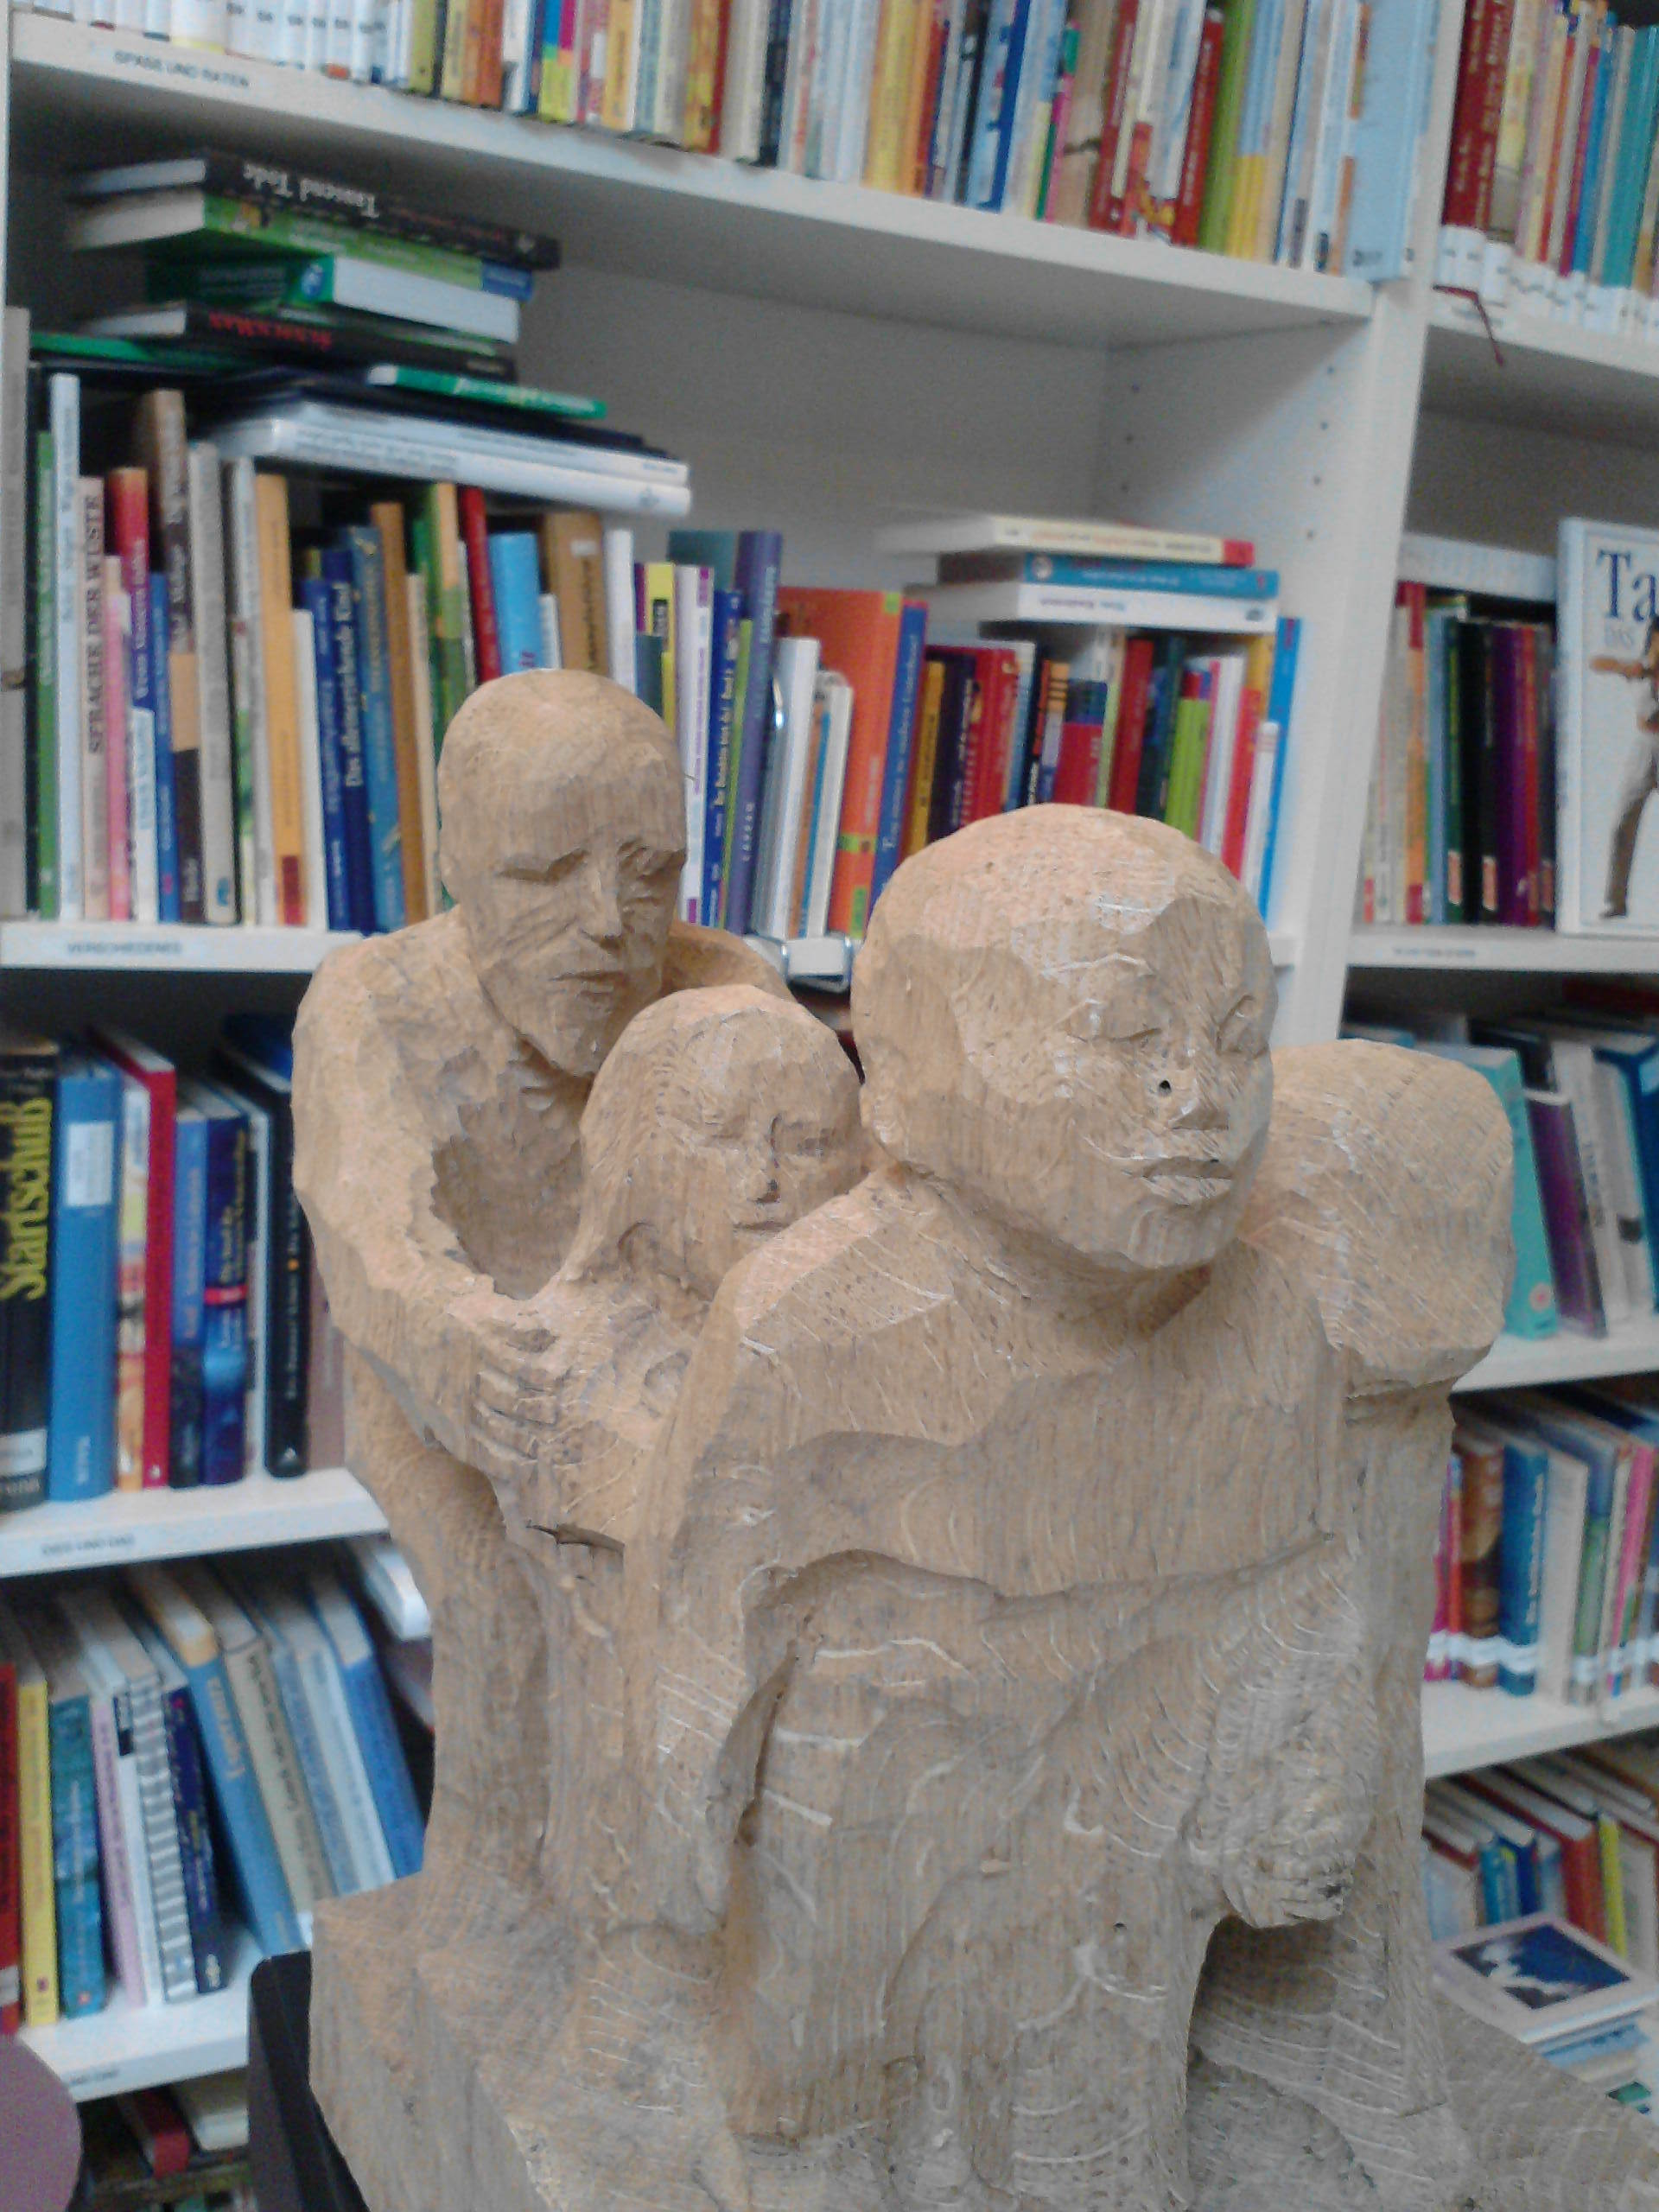
\includegraphics{img/abbildung1.jpg}
%\caption{}
\end{figure}

\section*{\texorpdfstring{\enquote{Ich finde nicht die richtigen
Worte}}{Ich finde nicht die richtigen Worte}}\label{ich-finde-nicht-die-richtigen-worte}

In ihrem Buch \enquote{Ich finde nicht die richtigen Worte}\footnote{Winkelheide,
  Marlies (2014): Ich finde nicht die richtigen Worte. Vechta: Geest}
hat Marlies Winkelheide mit eigenen Gedanken und Stimmen von Eltern und
Jugendlichen Eindrücke, Erfahrungen und Fragen aus ihrer
jahrzehntelangen Arbeit mit Geschwistergruppen gesammelt und assoziativ,
inspirierend, nachdenklich, fragend nebeneinander gestellt:

\begin{quote}
\enquote{Es ist für mich wichtig, einen geschützten Raum zu haben, in
dem man über alles reden kann, wenn man Probleme mit den Eltern oder dem
Geschwisterkind hat. So ein Raum wäre beispielsweise die
Geschwisterbücherei, wo ich mit Marlies schon öfter über Probleme mit
meiner Familie gesprochen habe. In der Geschwisterbücherei steht
außerdem sehr viel Lektüre zu verschiedenen Bereichen von Menschen mit
Geschwistern mit Behinderung in verschiedenen Lebenslagen zur Verfügung,
was für mich äußerst ansprechend war. Zudem ist der Raum auch sehr
schön, um sich mit anderen zu unterhalten, da es ein komfortables Sofa
gibt, was einen zum Miteinander reden anregt. Die Bücher sollten je nach
Lebenslage geordnet werden, damit man einen guten Überblick erhält und
schnellen Zugriff hat.}\footnote{Winkelheide (2014), S. 76}
\end{quote}

beschreibt ein Jugendlicher dort seine Bücherei-Erfahrung. Und eine
andere ergänzt: \enquote{Ich persönlich finde die Auswahl der Bücher
immer sehr gut und habe selber schon in verschiedensten
Lebenssituationen aus diesen gelernt.}\footnote{Winkelheide (2014), S.
  80}

Vieles, was das Leben von Geschwistern in Familien mit Menschen mit
Behinderung prägt, wird hier diskutiert oder sucht nach Worten --
manchmal als ein Herantasten, ein Wahrnehmen auf unterschiedliche Weise.
Ein Ratgeber oder \enquote{Rezeptbuch} dafür, wie die Begleitung von
Geschwistern in besonderen Lebenssituationen gelingt, kann und soll das
Buch von Marlies Winkelheide bewusst nicht sein. Ein Raum für schnelle
Antworten ist auch die Bücherei nicht. Die Fragen lassen mancher
Weiterentwicklung ihren Weg und ihr Tempo -- und auch ein mutiges
\enquote{Ich weiß nicht} gehört manchmal dazu. So, wie bei Janusz
Korczak, dem Namensgeber der Bücherei -- aber dazu später\ldots{}

\enquote{Hier geht es um {[}die Kinder{]} und staunend nehmen sie zur
Kenntnis, wie ernsthaft und vielfältig sich viele Autoren mit der
Situation der Kinder auseinandersetzen}, schrieb ein Vater ins
Gästebuch, das in der Bücherei ausliegt. Stimmen wie diese bringen zum
Ausdruck, dass die Besonderheit der Bücherei auch, jedoch nicht allein,
in dem speziellen Sammelauftrag für Bücher zu ausgewählten Lebensthemen
liegt. Entscheidend und prägend für das, was hier geschieht, ist vor
allem die Haltung, mit der sich Menschen mit und zwischen diesen Büchern
begegnen: Wer mag, kann in dem thematisch sortierten Präsenzbestand
stöbern, kann sich mit anderen über Gelesenes austauschen oder die
Denkanstöße und Fantasien, die durch Geschichten angeregt werden, erst
mal für sich behalten, in Gedanken bewegen und vielleicht irgendwann auf
irgendeine Weise zum Ausdruck bringen.

Nicht zufällig trägt dieser Ort den Namen jenes Mannes, der genau dieses
feine Wechselspiel, die immer wieder zu suchende Balance zwischen den
Geschichten der Bücher und den Geschichten des eigenen Lebens gesucht,
geschützt und beschrieben hat: Janusz Korczak.

\begin{figure}
\centering
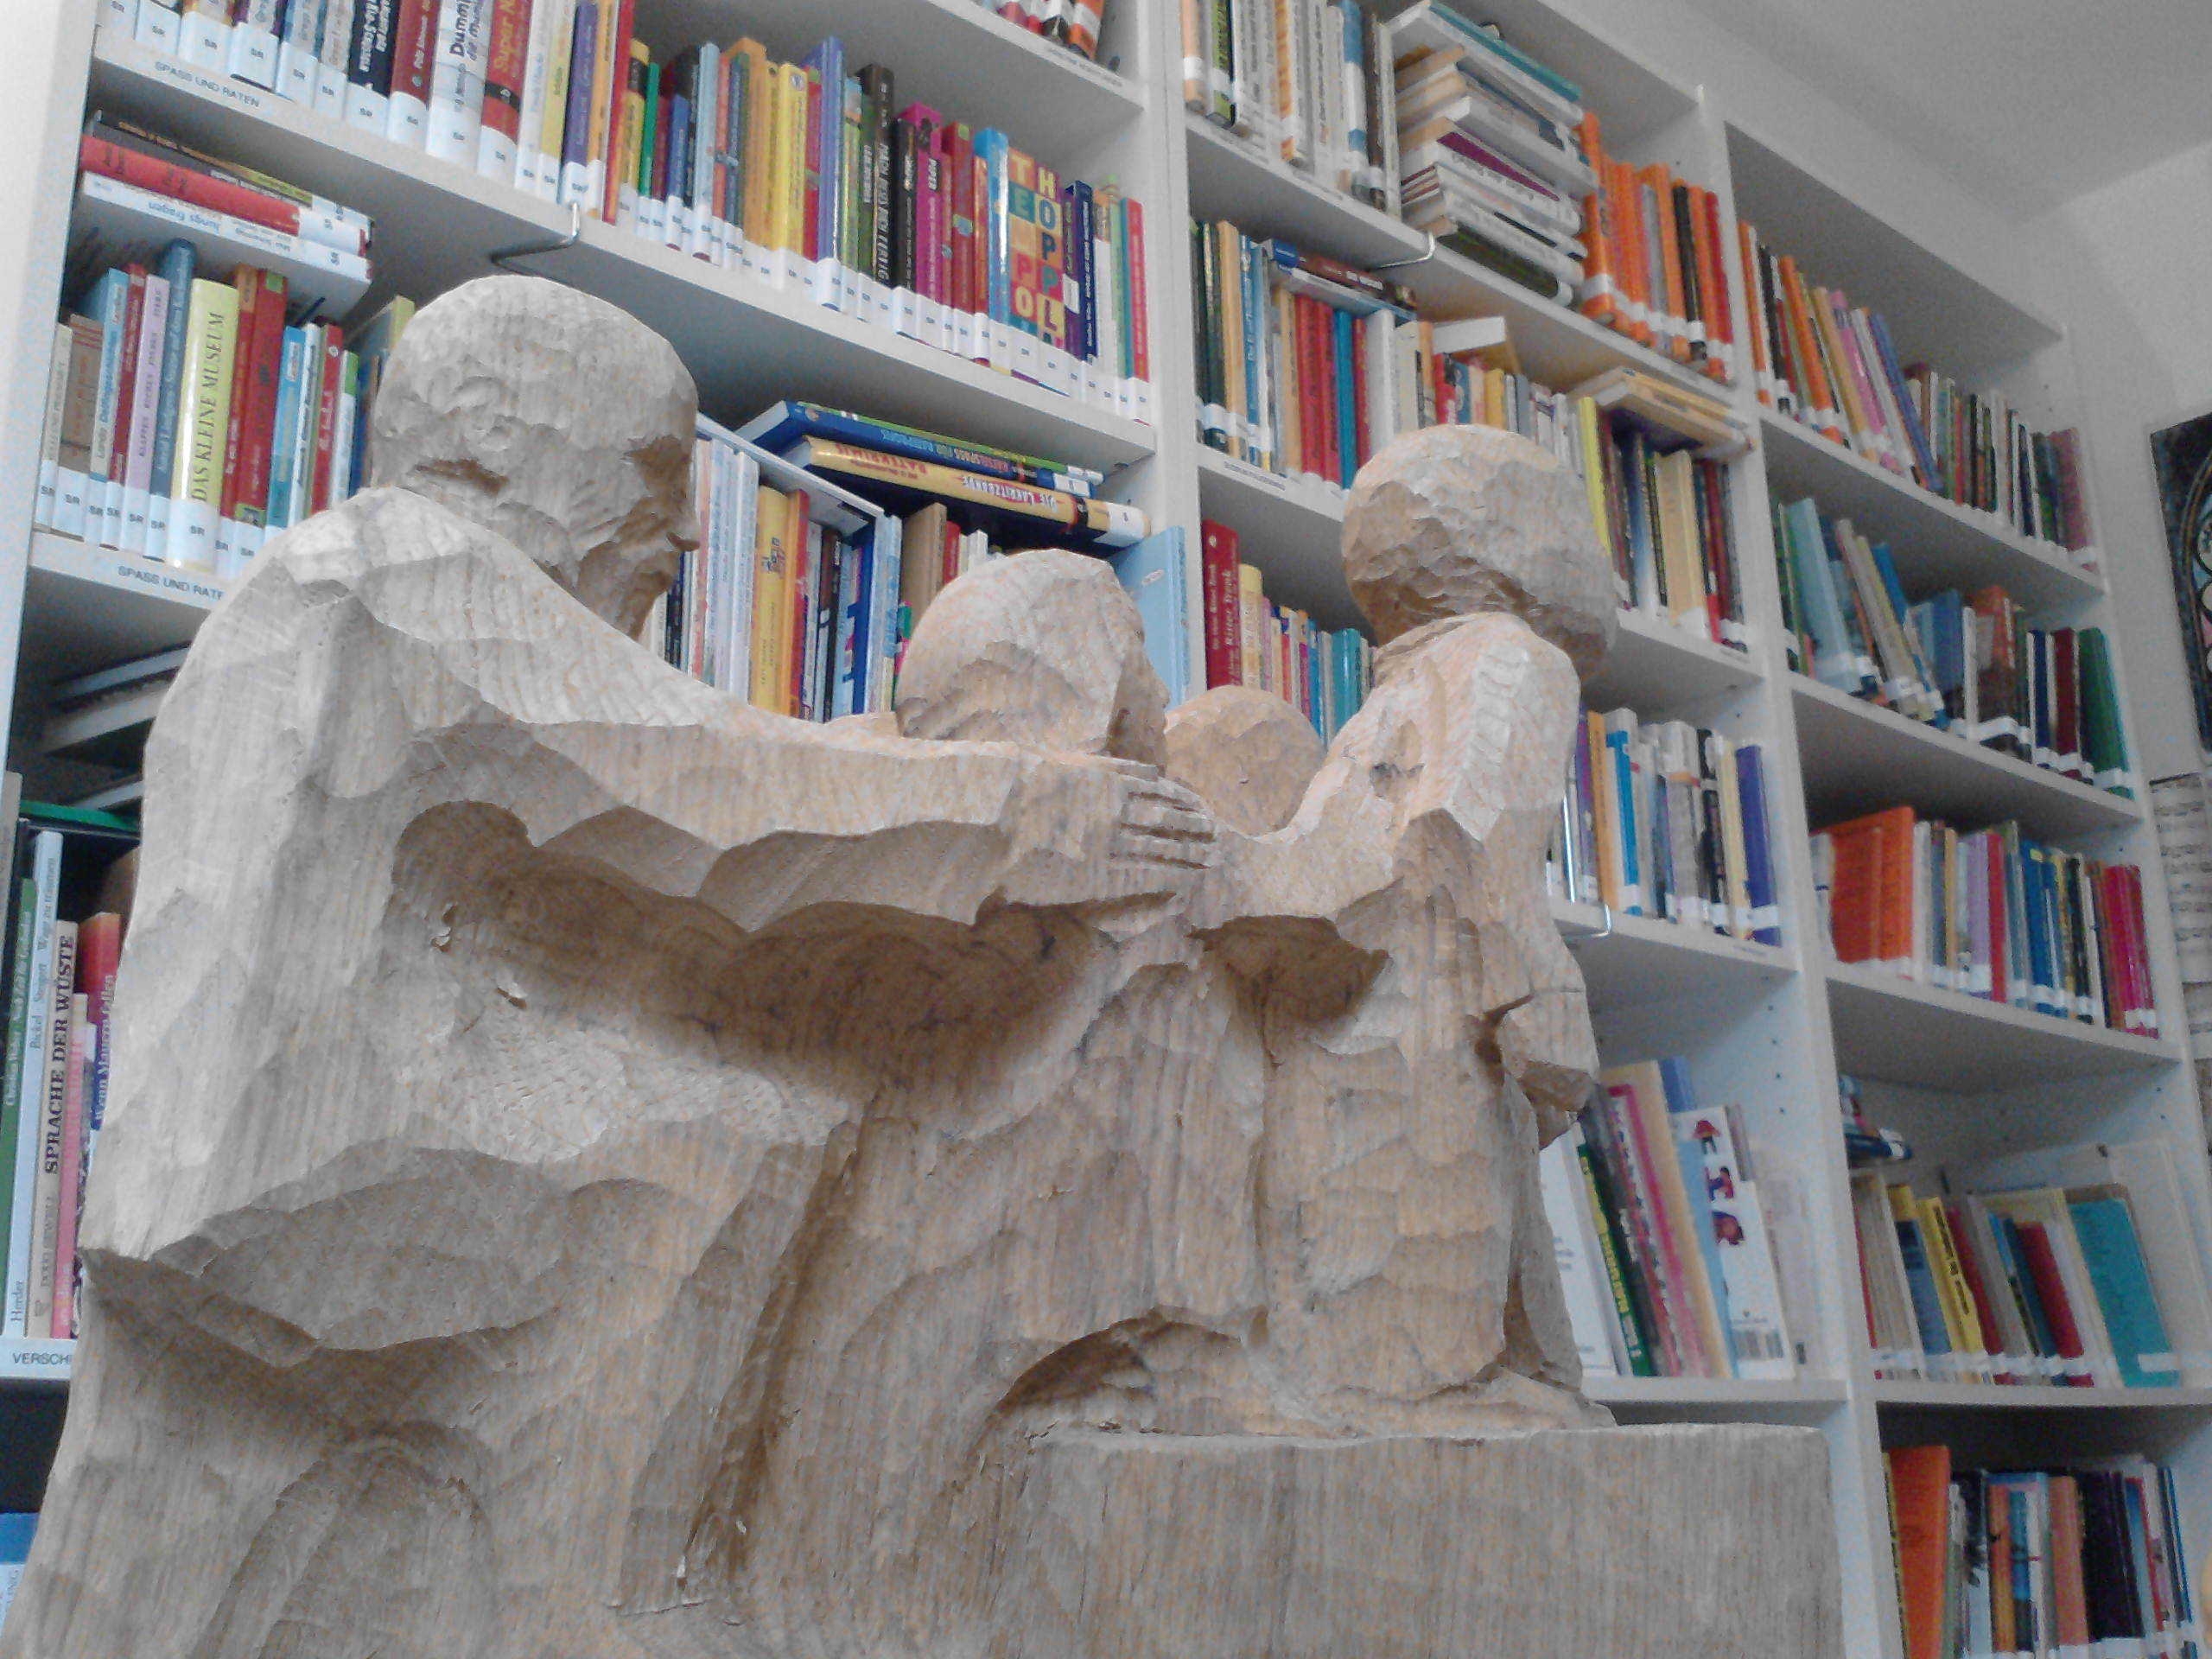
\includegraphics{img/abbildung2.jpg}
%\caption{}
\end{figure}

\section*{\texorpdfstring{\enquote{Ein Dichter -- das ist ein
Mensch, der starke Gefühle
hat}}{Ein Dichter -- das ist ein Mensch, der starke Gefühle hat}}\label{ein-dichter-das-ist-ein-mensch-der-starke-gefuxfchle-hat}

Viele denken bei dem Namen Janusz Korczak (1878-1942) zunächst an den
Waisenhausleiter im Warschauer Ghetto. Unvergessen ist, dass er im
August 1942 mit seinen Waisenkindern in Treblinka ermordet wurde. Im
Blick auf dieses grauenhafte Ende treten frühere Phasen, rücken andere
Aspekte seines Lebens eher in den Hintergrund. Janusz Korczak in allen
Facetten seines Wesens und Wirkens zu erfassen - das scheint ohnehin
kaum möglich zu sein. Manches lässt sich annähernd beschreiben, anderes
bleibt skurril oder rätselhaft: Er dachte und handelte, forschte, sprach
und schrieb als Sozialarbeiter, Psychologe, Philosoph, Theologe, Arzt,
Journalist, Dramatiker, Geschichtenerzähler und Kinderbuchautor. Was
seinen Beruf und seine Veröffentlichungen betrifft, scheint er sich
herkömmlichen Festschreibungen und eindeutigen Zuordnungen zu entziehen.
Alle genannten Fachdisziplinen sind für sein Leben und Werk von
Bedeutung, doch keine reicht aus, um seiner Vielschichtigkeit angemessen
gerecht zu werden.

Sechzehn dicke Bände umfasst die Ausgabe seiner sämtlichen Werke, die
inzwischen vollständig in deutscher Übersetzung vorliegt und in drei
Abteilungen das gesamte Spektrum der zu Papier gebrachten Aufzeichnungen
dokumentiert: Radiomanuskripte, Feuilletons, Essays, Momentaufnahmen,
Romane, Erzählungen, Briefe und das Tagebuch.\footnote{Korczak, Janusz
  (1998ff.): Sämtliche Werke. Ediert von Friedhelm Beiner und Erich
  Dauzenroth. Gütersloh: Gütersloher Verlagshaus}

Von Janusz Korczak lernen heißt vor allem: sich von ihm zu einer
besonderen Wahrnehmungs- und Handlungsweise inspirieren, für ein
besonderes Empfinden in der lebendigen Begegnung mit Kindern
sensibilisieren zu lassen. Gerade in den verschiedenen Vorlese- und
Erzählsituationen mit Büchern und Geschichten spielt für Korczak das
einzelne Kind als Individuum mit seinen ganz persönlichen Interessen und
Gefühlen, seinem Bedürfnis nach Nähe wie nach Rückzug und Für-sich-sein
eine besondere Rolle.\footnote{Vgl. dazu: Brandt, Susanne (2010):
  Gedankenflüge ohne Illusion. Janusz Korczak als Impulsgeber für die
  dialogische Begegnung mit Kindern beim Vorlesen, Erzählen und
  Schreiben. Mit einem Beitrag von Michael Kirchner. Wetzlar: Zentrum
  für Literatur (Schriftenreihe des Zentrums für Literatur in der
  Phantastischen Bibliothek Wetzlar; 10)}

\enquote{Es ist angenehm zu lesen, dass ein anderer ebenso denkt, ebenso
fühlt, dass andere auch traurig sind, glauben, träumen und
streben}\footnote{Korczak (1998ff.), Bd. 14, S. 570} schreibt er an
einer Stelle über die Wirksamkeit des Lesens zur Stärkung von Empathie
füreinander wie zum Umgang mit den eigenen Gefühlen.

\enquote{Alle Kinder sind Dichter, denn ein Dichter -- das ist ein
Mensch, der starke Gefühle hat, der heftig liebt und sich heftig
erzürnt, der ein starkes Wollen hat und ein starkes
Nichtwollen,}\footnote{Korczak (1998ff.), Bd. 14, S. 135} so heißt es
bei Korczak, der immer wieder auch das eigene Schreiben der Kinder
anzuregen wusste, an einer anderen Stelle.

Kinder sind Dichter -- das ist in der Janusz-Korczak-Geschwisterbücherei
ganz konkret zu verstehen, vor allem in Verbindung mit zahlreichen
Buchprojekten, die hier zur Umsetzung kommen wie zum Beispiel die
aktuelle Broschüre \enquote{Biete Erfahrung -- suche Haltung}.\footnote{Biete
  Erfahrung -- suche Haltung (2016). Hrsg. von Marlies Winkelheide mit
  dem Geschwisterrat. Vechta: Geest} In dieser Veröffentlichung werden
wohltuende wie schmerzliche Erfahrungen mit Sprache thematisiert: Worte,
durch die das Kind, der Jugendliche sich verletzt fühlt, aber auch
Sätze, die Geschwister gerne einmal hören möchten von Menschen in der
Familie, in der Schule, von Freunden.\\
Deutlich wird mit der Publikation, dass niemand eigentlich erkennen
kann, wann man verletzt wird und dass sich nur sehr schwer zum Ausdruck
bringen lässt, welche Sätze aufbauend wirken.

Auseinandersetzungen mit solchen und anderen Themen zeigen einmal mehr:
Persönliche Gefühle und Erfahrungen stehen in einer engen Verbindung zu
dem, was sprachlich als Botschaft empfangen oder ausgedrückt wird.
Bücher und Geschichten spielen dabei eine große Rolle und berühren
zugleich immer wieder auch Erfahrungen, die durch andere Mittel und
Menschen ihre eigene Sprache suchen, durch passende Materialien und
Bilder vielleicht erst zur Sprache finden. Genau dafür bietet die
Geschwisterbücherei nicht nur gut bestückte Regale, sondern eben auch
einen geschützten Raum, in dem Menschen sich in vertrauter Atmosphäre
treffen können.

Unterstützung und Zeichen der Anerkennung und Verbundenheit für diese
Arbeit hat die Bücherei bereits durch zahlreiche namenhafte Autorinnen
und Autoren wie Kirsten Boie, Renate Welsh, Achim Bröger, Doris
Meißner-Johannknecht, Gudrun Pausewang, Mirjam Pressler, Klaus Kordon
oder Josef Reding bekommen. Getragen vom Verein Stimme e.V. bleibt sie
angewiesen auf Spenden von verschiedenen Seiten.

Noch einmal Janusz Korczak: \enquote{Immer, wenn du ein Buch aus der
Hand legst und beginnst, den Faden eigener Gedanken zu spinnen, hat das
Buch sein angestrebtes Ziel erreicht.}\footnote{Korczak (1998ff.), Bd.
  14, S. 10}

Vermutlich gilt das für viele Bücher, die in der
Janusz-Korczak-Geschwisterbücherei bereit stehen und immer wieder
unzählige Gedankenfäden ins Spiel bringen, in ganz besonderer Weise: Sie
alle können etwas in Gang setzen, was weit über die Bücher und die
Bücherei hinaus weist -- aber ohne die Bücher und den Ort, den sie hier
gefunden haben, vielleicht niemals so beginnen könnte.

Weiterführende und aktuelle Informationen zur Geschwisterbücherei wie
auch Spendenmöglichkeiten für den Erhalt dieser wichtigen Einrichtung
beim Verein Stimme e.V. sind hier zu finden:
\url{http://www.geschwisterbuecherei.de/}

%autor
\begin{center}\rule{0.5\linewidth}{\linethickness}\end{center}

\textbf{Susanne Brandt}, geb.1964 in Hamburg, Studium in
Bibliothekswesen und Kulturwissenschaften, Qualifikation
Rhythmisch-musikalische Erziehung und bibliotherapeutische
Weiterbildung, seit 1995 zahlreiche Buchveröffentlichungen und Beiträge
in Zeitschriften und Anthologien; ab 1987 Leiterin der Musikbibliothek
in Cuxhaven, ab 2000 Bibliotheksleiterin in
Westoverledingen/Ostfriesland, seit Juni 2011 Lektorin bei der
Büchereizentrale Schleswig-Holstein in Flensburg.

\end{document}
